
\coverchapter{Results}\label{ch:results}
The search method we have developed and the resulting bijections work between different domains. The problem, however, is the lack of maintained implementations of domains using \css{}. With \css{} being a product of a research group that is mainly interested in permutation patterns, unsurprisingly the most supported domain are permutations with \tsc{}. As a consequence, we will mostly demonstrate bijections found between permutation classes.

\section{Cross-domain successes}
There is a very simple example for words provided in repository for \css{}. A word over an alphabet $\Sigma$ is any sequence of elements from $\Sigma$. A pattern in a word is another word that occurs as a consecutive subsequence. This class can be described as a triple $\mathcal{W} = (p, \Sigma, A)$, where $p$ is a required prefix, $\Sigma$ is the alphabet and $A$ is the set of patterns to avoid. For example $(\varepsilon, \set{0,1}, \set{11})$ is the set of binary strings that avoid consecutive 1's, that is
\[
    (\varepsilon, \set{0,1}, \set{11}) = \set{\varepsilon, 0, 1, 00, 01, 10, 000, 001, 010, 100, 101, \dotsc}.
\]


The bijection search will easily find bijections between sets such as $(\varepsilon, \set{0,1}, \set{11})$ and $(\varepsilon, \set{a,b}, \set{bb})$, that are identical given a bijection of the letters of the alphabet. The same goes for the trivial sets $(\epsilon, \set{0}, \emptyset)$ and $\Av{12}$, where there is only a single element of each length. The implementation for words has few strategies and limited effort was allocated to finding bijections between words and permutation classes. We will demonstrate two such bijections in greater detail but there is a caveat that needs to be addressed.

Take, e.g., the class $\mathcal{W} = (\varepsilon, \set{a,b}, \emptyset)$. For any fixed length $n$, there are $2^n$ unique words as we have a choice between two letters for each position in any sequence. This produces the sequence $1, 2, 4, 8, 16, 32, 64, \dotsc$ while the permutation class, $\Av{231,321}$, has the sequence $1, 1, 2, 4, 8, 16, 32, \dotsc$ which is off by one. We could use $\textsf{Av}_{\geq1}(231,312)$ instead, which shares this sequence with the words if we start from $n=1$, but that brings another problem. Words of length $n$ would map to permutations of length $n+1$ while parallel specifications require atoms to match. What we can do instead, is place the top point of $\textsf{Av}_{\geq1}(231,312)$ and factor it out. That leaves us with a tiling root $\mathcal{T}$ where
\begin{align*}
    \Av{231,312} &\cong \set{\varepsilon} \sqcup \textsf{Av}_{\geq1}(231,312),\\
    \textsf{Av}_{\geq1}(231,312) &\cong \set{\point{0.1}}\times \textsf{Grid}(\mathcal{T}).
\end{align*}
The tiling in question here is
\[
    \mathcal{T} = \left((2,1), \set{2^{(0,0)}1^{(1,0)}, 21^{(1,0)}, 231^{(0,0)}, 321^{(0,0)}},\emptyset\right).
\]
Now we can find and construct bijections between $\mathcal{W}$ and $\textsf{Grid}(\mathcal{T})$. It will map the words to gridded permutations in $\mathcal{G}^{(2,1)}$ instead of $\mathcal{G}^{(1,1)}$, but there is a trivial bijection from these gridded permutations to permutations.

The other bijection found was between $\mathcal{W} = (\varepsilon, \set{0,1}, \set{11})$ and $\Av{231,312,321}$. These are counted by the Fibonacci numbers but here we have the same issue as before, with one sequence being off by one. We remedy this in the same way as before, leaving us with a tiling root that can be seen in \FigureRef{fig:fibpermoffbyone}. This tiling can have at most a single point in cell $(1,0)$ and if it includes one, it must be greater than all the points in cell $(0,0)$. We can map any such gridded permutation to a permutation with a trivial bijection. Given a gridded permutation of length $n$ that contains no point in cell $(1,0)$ we append $n+1$ to the underlying permutation. If it contains a point in $(1,0)$ we place $n+1$ immediately prior to the last element.

\TableRef{tab:wordtilmap} shows the bijection constructed for $n \in \set{0,1,2,3}$ and the corresponding permutation with the mapping described above. \FigureRef{fig:fibwordtree} and \FigureRef{fig:fibpermtree} show the two parallel specifications that were found. Note that there is an empty class in the specification for words.

\begin{figure}[ht!]
    \centering
    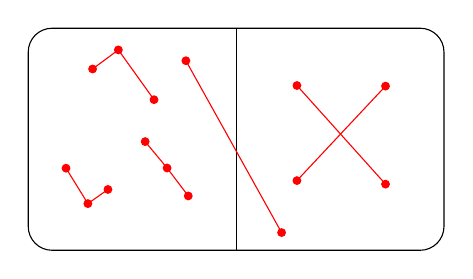
\begin{tikzpicture}[scale=1, every node/.style={scale=1}]
    \def\xscale{0.75} % Horizontal scale factor
    \def\yscale{0.75} % Vertical scale factor
    \def\spnt{0.075*0.75} % Size of smaller points
    \def\lpnt{0.125*0.75} % Size of larger points
    \draw (3.52*\xscale, 3.76*\yscale) -- (3.52*\xscale, 0);
    \draw[rounded corners=2ex] (0,0) rectangle (7.04*\xscale,3.76*\yscale);
    
    \fill[red] (4.55*\xscale, 1.18*\yscale) circle (\spnt);
    \fill[red] (6.05*\xscale, 2.78*\yscale) circle (\spnt);
    \draw[red] (4.55*\xscale, 1.18*\yscale) -- (6.05*\xscale,2.78*\yscale);
    
    \fill[red] (4.55*\xscale, 2.79*\yscale) circle (\spnt);
    \fill[red] (6.05*\xscale, 1.12*\yscale) circle (\spnt);
    \draw[red] (4.55*\xscale, 2.79*\yscale) -- (6.05*\xscale,1.12*\yscale);
    
    \fill[red] (2.67*\xscale, 3.21*\yscale) circle (\spnt);
    \fill[red] (4.29*\xscale, 0.3*\yscale) circle (\spnt);
    \draw[red] (2.67*\xscale, 3.21*\yscale) -- (4.29*\xscale,0.3*\yscale);
    
    \fill[red] (1.09*\xscale, 3.07*\yscale) circle (\spnt);
    \fill[red] (1.526001050877835*\xscale, 3.393088634545991*\yscale) circle (\spnt);
    \fill[red] (2.13*\xscale, 2.55*\yscale) circle (\spnt);
    \draw[red] (1.09*\xscale, 3.07*\yscale) -- (1.526001050877835*\xscale,3.393088634545991*\yscale) -- (2.13*\xscale,2.55*\yscale);
    
    \fill[red] (0.64*\xscale, 1.39*\yscale) circle (\spnt);
    \fill[red] (1.01*\xscale, 0.79*\yscale) circle (\spnt);
    \fill[red] (1.35*\xscale, 1.03*\yscale) circle (\spnt);
    \draw[red] (0.64*\xscale, 1.39*\yscale) -- (1.01*\xscale,0.79*\yscale) -- (1.35*\xscale,1.03*\yscale);
    
    \fill[red] (1.98*\xscale, 1.84*\yscale) circle (\spnt);
    \fill[red] (2.3511520552717013*\xscale, 1.3932029657051672*\yscale) circle (\spnt);
    \fill[red] (2.71*\xscale, 0.92*\yscale) circle (\spnt);
    \draw[red] (1.98*\xscale, 1.84*\yscale) -- (2.3511520552717013*\xscale,1.3932029657051672*\yscale) -- (2.71*\xscale,0.92*\yscale);
\end{tikzpicture}
    \caption{The tiling used instead of $\Av{231,312,321}$, to deal with the sequence offset of binary strings with no consecutive 1's.}
    \label{fig:fibpermoffbyone}
\end{figure}

\begin{table}[ht!]
    \centering
    \begin{tabular}{c|c|c}
    Word & Gridded permutation & Permutation\\
    \hline
    $\varepsilon$ & $\varepsilon$ & $1$\\
    $0$ & $1^{(0,0)}$ & $12$\\
    $1$ & $1^{(1,0)}$ & $21$\\
    $00$ & $12^{(0,0)}$ & $123$\\
    $01$ & $21^{(0,0)}$ & $213$\\
    $10$ & $1^{(0,0)}2^{(1,0)}$ & $132$\\
    $000$ & $123^{(0,0)}$ & $1234$\\
    $001$ & $213^{(0,0)}$ & $2134$\\
    $010$ & $132^{(0,0)}$ & $1324$\\
    $100$ & $12^{(0,0)}3^{(1,0)}$ & $1243$\\
    $101$ & $21^{(0,0)}3^{(1,0)}$ & $2143$\\
\end{tabular}
    \caption{An automated bijection up to $n=3$ between binary strings avoiding consecutive 1's and $\textsf{Grid}(\mathcal{T})$, where $\mathcal{T}$ is the tiling for $\textsf{Av}_{\geq1}(231,312,321)$ after placing and factoring out the top point. The corresponding permutation is also shown.}
    \label{tab:wordtilmap}
\end{table}

\begin{figure}
    \centering
    % TODO: Redo this crap properly 

{
\newcommand{\wordclass}[2]{%
\begin{tikzpicture}[scale=0.3, baseline=(current bounding box.center)]
\useasboundingbox (0,-3) rectangle (#1,3);
			\draw[thick, rounded corners=3pt] (0,0) rectangle (#1,3);
			\node at ({#1/2}, 1.5) {#2};
;
			    \end{tikzpicture}
}
    \begin{center}
    \scalebox{1}{\begin{tikzpicture}[scale=0.8, every node/.style={scale=0.8}]
        \node (root) at (0, 0) {\wordclass{8}{$(\varepsilon,\set{0,1},\set{11})$}};
        \node (lvl_1_1) at (-4, -2.25) {\wordclass{8}{$(0,\set{0,1},\set{11})$}};
        \node (lvl_1_2) at (0, -2.25) {\wordclass{8}{$\set{\varepsilon}$}};
        \node (lvl_1_3) at (4, -2.25) {\wordclass{8}{$(1,\set{0,1},\set{11})$}};
        \node (lvl_2_1) at (-6, -4.5) {\wordclass{8}{$\set{0}$}};
        \node (lvl_2_2) at (-2, -4.5) {\wordclass{8}{$(\varepsilon,\set{0,1},\set{11})$}};
        \node (lvl_2_3) at (1, -4.5) {\wordclass{8}{$\set{1}$}};
        \node (lvl_2_4) at (4, -4.5) {\wordclass{8.5}{$(10,\set{0,1},\set{11})$}};
        \node (lvl_2_5) at (7, -4.5) {\wordclass{8.5}{$(11,\set{0,1},\set{11})$}};
        \node (lvl_3_1) at (2, -6.75) {\wordclass{8}{$\set{10}$}};
        \node (lvl_3_2) at (6, -6.75) {\wordclass{8.5}{$(\varepsilon,\set{0,1},\set{11})$}};
        \node (lvl_4_1) at (0, -9) {\wordclass{8}{$\set{1}$}};
        \node (lvl_4_2) at (4, -9) {\wordclass{8}{$\set{0}$}};
        \ptedge{(root)}{(-0.5,1.2)}{(lvl_1_1)}{(-0.5,1.3)}
        \ptedge{(root)}{(-0.5,1.2)}{(lvl_1_2)}{(-0.5,1.3)}
        \ptedge{(root)}{(-0.5,1.2)}{(lvl_1_3)}{(-0.5,1.3)}
        \ptedge{(lvl_1_1)}{(-0.5,1.2)}{(lvl_2_1)}{(-0.5,1.3)}
        \ptedge{(lvl_1_1)}{(-0.5,1.2)}{(lvl_2_2)}{(-0.5,1.3)}
        \ptedge{(lvl_1_3)}{(-0.5,1.2)}{(lvl_2_3)}{(-0.5,1.3)}
        \ptedge{(lvl_1_3)}{(-0.5,1.2)}{(lvl_2_4)}{(-0.5,1.3)}
        \ptedge{(lvl_1_3)}{(-0.5,1.2)}{(lvl_2_5)}{(-0.5,1.3)}
        \ptedge{(lvl_2_4)}{(-0.5,1.2)}{(lvl_3_1)}{(-0.5,1.3)}
        \ptedge{(lvl_2_4)}{(-0.5,1.2)}{(lvl_3_2)}{(-0.5,1.3)}
        \ptedge{(lvl_3_1)}{(-0.5,1.2)}{(lvl_4_1)}{(-0.5,1.3)}
        \ptedge{(lvl_3_1)}{(-0.5,1.2)}{(lvl_4_2)}{(-0.5,1.3)}
    \end{tikzpicture}}
    \end{center}
}
    \vspace*{-12.5mm}
    \caption{The grammar of the specification found for binary strings avoiding consecutive 1's.}
    \label{fig:fibwordtree}
\end{figure}
\begin{figure}
    \centering
    \input{graphics/fibpermtree}
    \vspace*{-14mm}
    \caption{The grammar of the specification found for $\textsf{Av}_{\geq1}(231,312,321)$ after placing and factoring out the top point.}
    \label{fig:fibpermtree}
\end{figure}

\section{Permutation classes}
\todo[inline,caption={}]{
\begin{itemize}
    \item Talk about symmetries and that we don't bother with them
    \item Maybe add a section on symmetries in background?
    \item Start by crossing of articles (can subsection on them)
    \item Simion\&Schmidt, etc [todo: find more]
    \item Dump remaining 
    \item Could maybe visualize the group of classes as graphs [at least one example]
    \item Deal with Av(very long list of patterns) in some sensible way
\end{itemize}
}
